
% Following our general analytical results on the correction of the ERM model with regard to the particle position distribution $r\mapsto \exp(-\beta\cdot U(r))$ we will now in the following section discuss an approximation method called \emph{hypernetted chain approximation} (HNC) to solve the Dyson Fixed Point equation provided in the one loop expansion. 

As a first implementation of the corrected ERM theory we will now discuss a simple repulsive spring function given by % \color{red} USE $\sigma$\color{black}
\[
    \R\ni r\mapsto
        f_a^{(\textit{num})}(r)
    = \begin{cases}
        1 & \text{for } r < a, \\
        0 & \text{else}.
    \end{cases} \implies
    \vcenter{\hbox{
        \begin{tikzpicture}
            \draw[->] (0,0) -- (2,0) node[right] {{\small $r$}};
            \draw[->] (0,0) -- (0,1.5) node[above] {{\small $f_a^{(\textit{num})}(r)$}};

            \draw[] (1,0.1) -- (1,-0.1) node[below] {{\small $a$}};
    
            \draw[thick, domain=0:1, smooth, variable=\x, YvesKlein] plot ({\x}, {1});
            \draw[thick, domain=1:2, smooth, variable=\x, YvesKlein] plot ({\x}, {0});
        \end{tikzpicture}
    }}
\]
This spring funciton is defined within a finite interaction distance $a\in\R_{>0}$ and is zero elsewhere. The physical application is the model of soft spheres, where overlapping spheres are repelled by a spring force. This model is used in the context of molecular dynamics simulations. \cite{Hansen_McDonald_1979} To derive the potential given by this interaction we use a technique already applied during the analytical derivation of the pair interaction function in D.\ref{mdef:PairInteractionFunction}, where $[N]^2\ni(i,j)\mapsto d_{i,j}:R\mapsto R_i - R_j$ came into play. Following the same approach we find for positions $R\in V_{d,N}$ the interaction potential
\[
    U_a^{(\textit{num})}(R) = \sum_{(i,j)\in[N]^2}\ubra{
        \begin{cases}
            \frac{1}{2}\cdot(\dabs{d_{i,j}(R)}{2} - a)^2 & \text{for } d_{i,j}(R) < a, \\
            0 & \text{else}.
        \end{cases}
    }{=:u_a(d_{i,j}(R))} 
    \implies
    \vcenter{\hbox{
        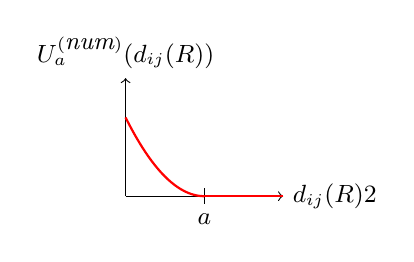
\begin{tikzpicture}
            \draw[->] (0,0) -- (2,0) node[right] {{\small $\dabs{d_{ij}(R)}{2}$}};
            \draw[->] (0,0) -- (0,1.5) node[above] {{\small $U_a^{(\textit{num})}(d_{ij}(R))$}};

            \draw[] (1,0.1) -- (1,-0.1) node[below] {{\small $a$}};
    
            \draw[thick, domain=0:1, smooth, variable=\x, red] plot ({\x}, {(\x - 1)^2});
            \draw[thick, domain=1:2, smooth, variable=\x, red] plot ({\x}, {0});
        \end{tikzpicture}
    }}
\]
Notice that for $a = 1$ we find the same form as \cite{Jacquin_2010}. To describe forces induced by the spring potential in $d$ dimensions in our system, we introduce radial symmetry by composing $f_a^{(\textit{num})}\circ\dabs{\cdot}{2}$ on any disctance $d_{ij}(R)$ of two particles $i,j$, i.e. we encode the isotropic character of the system into $f^{\textit{num}}_a$. With this we are now ready to calculate the particle probability density $R\mapsto {\exp}\bbra{-\beta\cdot U_a^{(\textit{num})}(R)}$ in the following.